\chapter{Philadelphia: Old Money and the Geometry of Wealth}

This episode begins in pursuit, not in exposition. We first hear the tip near the bank, the police-assisted identification, the half-playful claim that somebody ``looks like money,'' and only after that do we hear Philadelphia named as a city of old money and generational wealth. That order matters. It makes wealth feel hidden but nearby before it is described in the abstract. No validated board or diagram frame survives from this lecture, so every figure below is a cautious transcript-derived reconstruction rather than a transcription of visible mathematics. The underlying mathematics is nevertheless real. It appears in the host's access logic, in the filmmaker's insistence on ownership, in the private-equity operator's value-creation rule, in the dentists' account of compounding, and in the block owner's conservative use of bank leverage.

\section{Philadelphia as a Search Field}

We should keep the cold open in front of us, even though its chronology is not perfectly clean. The host is told that a man near the bank is rich, perhaps a billionaire. The first exchange is already about method. The host does not merely ask a question; he justifies the question by displaying credibility. He says he has grown the channel to roughly eighteen million followers and has interviewed thirty-one billionaires. Only after that local scene does the lecture widen and declare Philadelphia a special case: a city of very old money, dense private wealth, and eighteen resident billionaires.

Placed in the order in which the lecture itself places them, the framing numbers are
\begin{align}
F_{\text{host}} &= 18 \times 10^6,\\
N_{\text{billionaires interviewed}} &= 31,\\
N_{\text{billionaires,Philly}} &= 18.
\end{align}
These numbers do not yet explain how anyone became rich. What they explain is why the host expects the search to work at all. The lecture's premise is that access can be forced into existence by persistence plus recognized credibility.

One further feature of the opening should not be lost. Philadelphia is not first introduced as a spreadsheet of rich residents. It is introduced as a field in which wealth is hard to read from the outside. The host repeatedly uses visual inference---``you look like money''---but the lecture quickly teaches us that visual inference is only the opening move. The real work begins when visibility fails.

\section{Refusal, Credibility, and the First Opening}

Immediately after the city is announced, the lecture runs into friction. There is a corrupted stretch in the transcript, then a series of failed approaches, and then the first clear recap: Philly is tough, there is old money everywhere, and nobody wants to stop. At this point the host states the episode's first explicit mechanism: every no is one step closer to a yes.

A convenient reconstruction of the lecture's search logic is
\begin{equation}
\text{old-money field}
\to
\text{cold approach}
\to
\text{refusal}
\to
\text{credibility proof}
\to
\text{usable answer}.
\end{equation}
This is not a spoken formula. It is the simplest way to preserve what the lecture is doing structurally.

\begin{figure}[h]
\centering
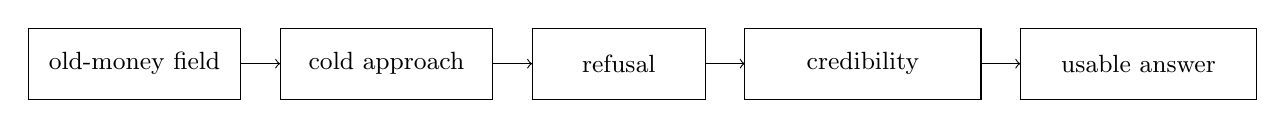
\begin{tikzpicture}[x=1cm,y=1cm]
\draw (0,0) rectangle (2.7,0.9);
\draw (3.2,0) rectangle (5.9,0.9);
\draw (6.4,0) rectangle (8.6,0.9);
\draw (9.1,0) rectangle (12.1,0.9);
\draw (12.6,0) rectangle (15.6,0.9);

\node at (1.35,0.45) {\small old-money field};
\node at (4.55,0.45) {\small cold approach};
\node at (7.5,0.45) {\small refusal};
\node at (10.6,0.45) {\small credibility};
\node at (14.1,0.45) {\small usable answer};

\draw[->] (2.7,0.45) -- (3.2,0.45);
\draw[->] (5.9,0.45) -- (6.4,0.45);
\draw[->] (8.6,0.45) -- (9.1,0.45);
\draw[->] (12.1,0.45) -- (12.6,0.45);
\end{tikzpicture}
\caption{Transcript-derived access funnel. The lecture treats refusal not as dead air but as part of the mechanism.}
\end{figure}

The recaps matter here. After the refusals, the host does not merely say that people walked away. He re-states the scene and extracts the rule. This is very much the lecture's rhythm: a bit of street-level noise, then a plain spoken compression of what the noise means.

\subsection{Question \& Answer}

\paragraph{Question.} If Philadelphia is so rich, why is it so hard to get anyone to stop and talk?

\paragraph{Answer.} Because wealth density and conversational accessibility are different things. A city may contain old money without exposing its doctrine on demand. The lecture insists on this by making access friction part of the pedagogy. In such a field, one does not merely find wealth; one has to penetrate its social shell.

From here the lecture needs a first real opening. It gets one when a passerby, initially guarded, recognizes the channel and agrees to talk. That change of state is important. The breakthrough does not come from luck alone. It comes from the exact mechanism the host has been advertising: credibility makes a reluctant conversation possible.

\section{Ownership After Rejection}

The filmmaker interview is the first long-form segment, and it is arranged with care. It begins commercially, not spiritually. The speaker says he has been in film for about twenty-five years, that he started his own company, and that the essential thing is ownership. The spoken rule is blunt enough that we may preserve it in the following compact form:
\begin{equation}
W_{\text{creative}} \uparrow
\qquad \text{when} \qquad
s_{\text{ownership}} \uparrow,
\end{equation}
where \(s_{\text{ownership}}\) stands for one's share of control and economic claim in the thing being made.

The money line in the transcript is noisy, but the safest quantitative note is still worth keeping:
\begin{equation}
t_{\text{film}} \approx 25\ \text{years},
\qquad
Y_{\max,\text{film}} \approx \$35 \times 10^6.
\end{equation}
We should treat the number cautiously. The point of the segment is not an audited earnings statement. The point is the speaker's sharp connection between scale and ownership.

\paragraph{Anecdote.} He is rejected at an audition, notices the producer, and suddenly sees the structure of the business. The producer, not the rejected actor, sits nearest to the economic center.

\paragraph{Claim.} Rejection need not mean that one has no place in the field. It may mean that one is standing in the wrong place inside the field.

\paragraph{Mechanism.} By moving from being selected to helping own the selection machinery, one changes the income channel itself. The lecture's commercial emphasis is not on artistry as such, but on claim over the asset being produced.

From this point the interview widens. The grandmother's remark---one is born looking like one's parents but dies looking like one's decisions---moves the conversation from ownership to path dependence. The speaker adds that things often get harder just before success. Then comes the bicycle metaphor. We should not mathematize that metaphor too aggressively; its role is motivational. But the logical shape is clear enough:
\begin{equation}
\text{rejection}
\to
\text{repositioning}
\to
\text{ownership}
\to
\text{persistence}.
\end{equation}

Faith is then introduced not as ornament, but as part of the speaker's explanation for endurance. The sequence matters. Ownership comes first, then persistence, then faith as the thing that stabilizes persistence when the climb steepens.

Finally, the speaker supplies a second, more social mechanism. Clarence Avant's advice is to keep a favor book. Some people helped you and will be forgotten unless you remember; others never helped and will be first in line when favors are distributed. The closing maxim, ``never mistake attendance for alliance,'' completes the segment. The lecture has moved from economic ownership to alliance selection. Both are forms of choosing the right locus of control.

\subsection{Question \& Answer}

\paragraph{Question.} How does rejection become a push toward ownership rather than a reason to stop?

\paragraph{Answer.} The lecture's answer is that rejection can disclose where the real control sits. Once the speaker sees that the producer occupies the commanding point in the business, rejection stops being only a wound and becomes information. The field has told him where value lives.

The host's recap after this interview is also part of the substance. He says it was one of the best interviews he has done and, crucially, reminds us that the man did not want to talk at first. ``Credibility kills all bad attitudes'' is not a theorem, but in this episode it functions like one. It is the hinge that carries us from refusal into doctrine.

\section{Private Equity, Value Creation, and Boring Businesses}

The lecture now changes register. After a segment filled with aphorism and social intelligence, we move into a cleaner mechanics section with the private-equity-and-sports owner. The path into the interview is itself telling. The host again begins with surface cues---``you look like money''---but the conversation quickly abandons appearance and becomes a miniature seminar in value creation.

The numerical anchors are straightforward:
\begin{align}
t_{\text{PE}} &\approx 20\ \text{years},\\
A_{\text{managed}} &\approx \$80 \times 10^9,\\
I_{\text{seed}} &\approx \$2{,}000.
\end{align}
The last quantity is the bar-mitzvah money placed into real estate under a mentor's guidance. It matters because the lecture is careful to tie very large outcomes to surprisingly small but structured beginnings.

Before he explains private equity, the speaker makes a useful distinction about temperament. Not everyone is built for entrepreneurship. Some people can be entrepreneurial inside someone else's business. That remark belongs in this section because it prevents the lecture from collapsing into a crude founder mythology. Wealth here is connected to value creation, not to a single romantic identity.

When the host asks for a third-grade explanation of private equity, the speaker gives the lecture's cleanest two-lane model. We may preserve it in words first:
\begin{enumerate}
\item buy a broken business and fix it, then sell or continue to own the improved thing;
\item back a business already on the upswing, but lacking capital and know-how.
\end{enumerate}
In either lane, the minimum business claim is
\begin{equation}
V_{\text{after}} > V_{\text{before}}.
\end{equation}
The lecture never suggests that capital earns by mere passivity. Capital must be joined to repair, operational skill, or scaling knowledge.

\begin{figure}[h]
\centering
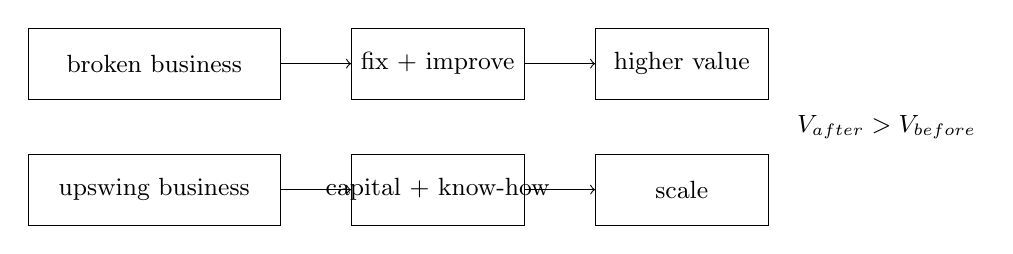
\begin{tikzpicture}[x=1cm,y=1cm]
\draw (0,1.6) rectangle (3.2,2.5);
\draw (4.1,1.6) rectangle (6.3,2.5);
\draw (7.2,1.6) rectangle (9.4,2.5);

\draw (0,0) rectangle (3.2,0.9);
\draw (4.1,0) rectangle (6.3,0.9);
\draw (7.2,0) rectangle (9.4,0.9);

\node at (1.6,2.05) {\small broken business};
\node at (5.2,2.05) {\small fix + improve};
\node at (8.3,2.05) {\small higher value};

\node at (1.6,0.45) {\small upswing business};
\node at (5.2,0.45) {\small capital + know-how};
\node at (8.3,0.45) {\small scale};

\draw[->] (3.2,2.05) -- (4.1,2.05);
\draw[->] (6.3,2.05) -- (7.2,2.05);
\draw[->] (3.2,0.45) -- (4.1,0.45);
\draw[->] (6.3,0.45) -- (7.2,0.45);

\node at (10.9,1.25) {\small \(V_{\text{after}} > V_{\text{before}}\)};
\end{tikzpicture}
\caption{Transcript-derived two-lane private-equity schematic.}
\end{figure}

The speaker then makes an unexpectedly important move. He prefers boring businesses. While everybody is talking about AI, he points to plumbing, electrical work, construction, and other service businesses that cannot be automated away by conversational glamour. This is a recurring motif across the broader series, and it appears here in a particularly crisp form: sexy narratives attract attention, but unsexy businesses often hold the harder cash flows.

Real estate sits naturally beside this claim. The speaker calls it a long-term hard-asset business and immediately gives the key mechanism:
\begin{equation}
\text{tenant rent}
\to
\text{debt service}
\to
\text{mortgage paydown}.
\end{equation}
The transcript alternates between ``paying down your mortgage'' and ``reducing your debt service.'' We need not force a finer accounting than the speaker intends. His point is that the asset's users carry the financing burden.

Leverage, he says, is everything, though too much leverage is dangerous. This double statement matters. The lecture praises leverage only in the same breath in which it limits leverage.

The section closes on another asymmetry:
\begin{equation}
t_{\text{build rep}} \approx 20\ \text{years},
\qquad
t_{\text{destroy rep}} \approx 5\ \text{minutes}.
\end{equation}
Reputation is treated here almost like a financial asset with a deeply asymmetric volatility profile. It accumulates slowly, and a single bad act can wipe it out. The host's earlier credibility talk and the block owner's later bank trust both rhyme with this relation.

\subsection{Question \& Answer}

\paragraph{Question.} How does private equity actually make money?

\paragraph{Answer.} The lecture's answer is disarmingly plain. We either repair a damaged asset or accelerate a promising one. In both cases we add something the asset does not yet have---operating discipline, experience, capital, or scale---and we are paid through the increase in value that follows.

We should also keep one final beat from this interview. The speaker says that after a certain point it is not really about money. It is about building, solving, backing ideas, and caring for employees and their families. In this lecture, commercial mechanics and life motive are repeatedly braided together rather than kept in separate chapters.

\section{Access as an Interruption}

At this point the lecture deliberately breaks its own rhythm. The host now tells us that billionaires made him a millionaire at twenty-three, that he built a multimillion-dollar business by interviewing them, and that access changes everything. He turns the episode's social mechanism into a marketed offer: live calls, billionaire mentorship, direct questions, no replay.

We should keep this interruption short but visible. Its function is structural. After the private-equity segment has shown that access can deliver serious commercial doctrine, the host monetizes access itself. In that sense the sponsor block is not external to the episode. It is the episode's method turned into product form.

But the lecture does not let that become the center. The interruption prepares a contrast. If access is valuable, then what exactly is it valuable \emph{for}? The answer arrives immediately afterward: not for spectacle alone, but for mechanisms that survive after the microphone is gone. The next segment, with two retired dentists, returns us to the slowest and perhaps most durable mechanism in the entire episode.

\section{The Dentists and the Long Flat Part of Compounding}

The dentists are explicit from the start: they did not get wealthy pulling teeth. They earned money in dentistry, but wealth came from what they did with the money afterward. The prescription is concrete and repetitive on purpose: take the money earned from dentistry, or from YouTube, put it into Vanguard index funds, and do it for decades.

\paragraph{Anecdote.} Two classmates from more than forty years ago are now retired, relaxed, and clearly living from a stock of accumulated wealth rather than from daily labor.

\paragraph{Claim.} Income is not yet wealth. Wealth appears when earnings are repeatedly converted into invested capital.

\paragraph{Mechanism.} The relevant engine is compounding, not mere saving.

A clean mathematical rendering of the speaker's linear-versus-geometric contrast is
\begin{equation}
W_{\text{lin}}(t) = W_0 + at,
\qquad
W_{\text{geom}}(t) = W_0(1+r)^t.
\end{equation}
These formulas are a standard reconstruction, not a board transcription. But they preserve the speaker's central intuition exactly: linear growth adds the same amount each period, whereas geometric growth scales with the size already achieved.

A slightly richer reconstruction of the dentists' logic tracks invested capital rather than total wealth:
\begin{equation}
K_{t+1} = (1+r)K_t + (Y_t - C_t).
\end{equation}
Here \(K_t\) is the invested pool, \(Y_t\) is earned income, and \(C_t\) is consumption. The lecture's warning about overspending is simply the statement that the contribution term \(Y_t-C_t\) can be choked off before the compounding regime ever becomes visible.

Let us work one short example because the lecture itself insists on the shape of the curve, not just the slogan. Suppose the yearly investable surplus is a constant
\begin{equation}
s = Y_t - C_t,
\qquad
K_0 = 0.
\end{equation}
Then
\begin{align}
K_1 &= s,\\
K_2 &= (1+r)s + s,\\
K_3 &= (1+r)^2 s + (1+r)s + s.
\end{align}
We recognize a geometric sum. Thus
\begin{equation}
K_t = s \sum_{j=0}^{t-1}(1+r)^j
= s\,\frac{(1+r)^t - 1}{r}.
\end{equation}
This formula is not spoken in the interview, but it is exactly the cleaned mathematical content of the dentist's verbal picture. For a long time the curve looks almost inert, because the base is still small. Later the multiplicative term takes over. Indeed,
\begin{equation}
K_{t+1} - K_t = rK_t + s.
\end{equation}
Early on, the increment is mostly the steady contribution \(s\). Later on, the term \(rK_t\) dominates. That is the entire mystery of the ``flat for a long time, then explodes upward'' description.

\begin{figure}[h]
\centering
\begin{tikzpicture}[x=0.9cm,y=0.6cm]
\draw[->] (0,0) -- (11,0);
\draw[->] (0,0) -- (0,7);

\node at (10.7,-0.45) {\small time \(t\)};
\node at (-0.45,6.8) {\small wealth};

\draw (0.5,0.55) -- (9.6,4.05);
\node at (8.85,3.45) {\small linear};

\draw[smooth] plot coordinates {(0.5,0.18) (1.8,0.28) (3.0,0.45) (4.2,0.72) (5.4,1.18) (6.4,1.95) (7.2,3.0) (8.0,4.35) (8.7,5.8) (9.2,6.7)};
\node at (7.7,6.25) {\small geometric};

\draw[dashed] (4.9,0) -- (4.9,1.1);
\node at (4.9,-0.55) {\small long flat part};
\end{tikzpicture}
\caption{Transcript-derived compounding sketch. The key verbal claim is that invested wealth seems inert for a long time and then accelerates sharply.}
\end{figure}

\subsection{Question \& Answer}

\paragraph{Question.} Why does invested money seem to do almost nothing for a long time and then suddenly accelerate?

\paragraph{Answer.} Because compounding is proportional to the stock already accumulated. When the stock is small, the return term is visually unimpressive. When the stock is large, the same rate acts on a large base and the curve appears to wake up. The law did not change; only the size of the base changed.

The dentists immediately attach a moral and sociological corollary to this mathematics. Young people spend too much. Instant gratification moves consumption upward and starves the contribution term. Starting early matters because time is needed to get through the flat part before the curve turns upward.

The host then folds himself back into the lecture as a generational counterpoint. He claims a business doing about six million dollars this year and about seven hundred thousand dollars last month:
\begin{equation}
Y_{\text{host,year}} \approx \$6 \times 10^6,
\qquad
Y_{\text{host,last month}} \approx \$0.7 \times 10^6.
\end{equation}
These are not here to overthrow the dentists' lesson. They are here to complicate it. The lecture now carries two time scales at once: the slow compounding of invested surplus, and the faster scale of content-driven cash flow. Yet even the faster path is immediately tied, in the host's own story, to mentors, relocation, and entering a place like Austin where growth-oriented people gather. Fast money is not presented as magic. It too has structure.

The older speaker's closing remarks in this segment widen the frame again. Life is not fair, and life is not a straight line. One has ups and downs. Parents and mentors are often recognized only after the fact. These are not equations, nor should we force them into equations. But they belong here because they explain why the compounding section does not remain a sterile finance lesson. It is a lesson about time, delay, and recognition.

\section{The Block, the Bank, and Conservative Leverage}

The final interview returns us to the street and to concrete property. The speaker gestures to the block and says he owns from one corner to the next. The question is immediate and practical: how does one get enough money to buy buildings on that scale?

The first answer is only two words long: friendly banks. But the lecture does not leave the answer there. Friendly banks are not a mysterious gift. They are the consequence of a history. The speaker says he paid back the banks, behaved conservatively, and tried to pay back more principal per year than was required. A cautious mathematical rendering of that discipline is
\begin{equation}
D_{t+1} = D_t - P_{\text{sched}} - P_{\text{extra}},
\end{equation}
where \(D_t\) is debt outstanding, \(P_{\text{sched}}\) is the scheduled principal reduction, and \(P_{\text{extra}}\) is the additional principal voluntarily retired.

The financing split is then given in the lecture's simplest usable form:
\begin{equation}
V = E + D,
\qquad
\frac{E}{V} \approx 0.3,
\qquad
\frac{D}{V} \approx 0.7.
\end{equation}
That is, roughly thirty percent equity and seventy percent bank debt. The speaker also says that sometimes the equity for a new acquisition came by leveraging existing real estate. In the mildest notation,
\begin{equation}
E_{\text{new deal}}
\text{ can be supplied partly by pledging }
E_{\text{old real estate}}.
\end{equation}

\begin{figure}[h]
\centering
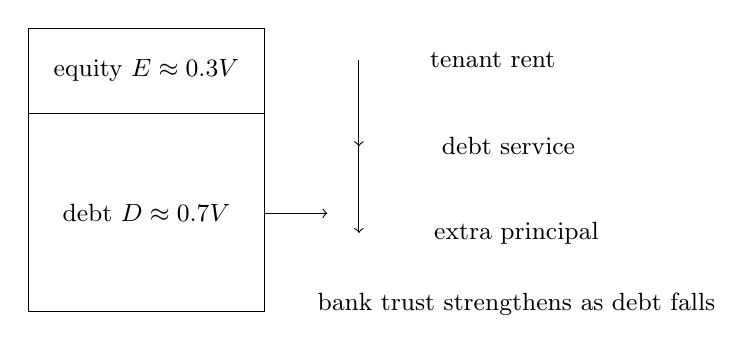
\begin{tikzpicture}[x=1cm,y=1cm]
\draw (0,0) rectangle (3,3.6);
\draw (0,0) rectangle (3,2.52);
\node at (1.5,1.25) {\small debt \(D \approx 0.7V\)};
\node at (1.5,3.06) {\small equity \(E \approx 0.3V\)};

\draw[->] (4.2,3.2) -- (4.2,2.1);
\draw[->] (4.2,2.1) -- (4.2,1.0);
\node at (5.9,3.2) {\small tenant rent};
\node at (6.1,2.1) {\small debt service};
\node at (6.2,1.0) {\small extra principal};

\draw[->] (3.0,1.25) -- (3.8,1.25);
\node at (6.2,0.1) {\small bank trust strengthens as debt falls};
\end{tikzpicture}
\caption{Transcript-derived capital-stack and cash-flow schematic for the final real-estate interview.}
\end{figure}

\subsection{Question \& Answer}

\paragraph{Question.} How does a bank keep trusting an operator enough to finance more property?

\paragraph{Answer.} By observing a conservative repayment history. In the lecture's own language, the operator pays back the banks, pays down principal aggressively, and makes himself legible as a good client. Bank trust is thus not a mood. It is memory encoded in lending behavior.

The episode then gives the final real-estate segment a motive beyond accumulation. The speaker says he wanted to build a tremendous community, to place great tenants in the properties, and to create an environment people would enjoy. The block is not described merely as a rent machine. It is described as a shaped piece of city life.

Failure also returns here in a final, compressed form. Everyone has failures, even every day and every hour. The danger is not failure itself but dwelling in it. That remark belongs exactly where the lecture puts it, beside leverage and scale. The commercial machine is never represented as frictionless.

The close is characteristic of the whole episode. We do not end on capitalization rates or on the number of buildings. We end on family, regret, and faith. The speaker says to spend as much time as possible with family. He recalls losing his brother. Prayer and care for family are offered as the thing that carries one through rock-bottom periods. Thus the lecture returns, at the end, to the same braid it has maintained all along: business mechanism, personal endurance, and life structure.

\section{Summary}

The chapter unfolds exactly as the lecture unfolds. First wealth is sensed before it is defined: a tip, a bank, a rich-looking stranger, a city of hidden old money. Then refusal teaches the first mechanism, namely that access is a problem in its own right and that credibility is one way of solving it. The filmmaker turns rejection into an ownership lesson. The private-equity operator turns value creation into a two-lane model and prefers boring businesses over glamorous ones. The sponsor interruption reminds us that access has itself become a commodity. The dentists then supply the clearest mathematics in the episode: invested money grows geometrically, not linearly, and the decisive region of the curve arrives only after a long flat beginning. Finally, the block owner turns leverage into street-level practice: conservative borrowing, principal reduction, recycled equity, bank trust, community, failure, family.

What emerges is not a single doctrine but a family of related ones. Ownership matters. Value must be created, not merely admired. Reputation compounds slowly and can be destroyed quickly. Real estate works when leverage is disciplined. Compounding works when spending does not suffocate investing. And none of these mechanisms stands outside life. The lecture ends, as it should, not with a formula alone but with the reasons one would want the formula to work.